\documentclass[]{book}
\usepackage{lmodern}
\usepackage{amssymb,amsmath}
\usepackage{ifxetex,ifluatex}
\usepackage{fixltx2e} % provides \textsubscript
\ifnum 0\ifxetex 1\fi\ifluatex 1\fi=0 % if pdftex
  \usepackage[T1]{fontenc}
  \usepackage[utf8]{inputenc}
\else % if luatex or xelatex
  \ifxetex
    \usepackage{mathspec}
  \else
    \usepackage{fontspec}
  \fi
  \defaultfontfeatures{Ligatures=TeX,Scale=MatchLowercase}
\fi
% use upquote if available, for straight quotes in verbatim environments
\IfFileExists{upquote.sty}{\usepackage{upquote}}{}
% use microtype if available
\IfFileExists{microtype.sty}{%
\usepackage{microtype}
\UseMicrotypeSet[protrusion]{basicmath} % disable protrusion for tt fonts
}{}
\usepackage[margin=1in]{geometry}
\usepackage{hyperref}
\hypersetup{unicode=true,
            pdftitle={Rapid Watershed Assessment Using FluvialGeomorph},
            pdfauthor={Michael Dougherty, Chris Haring, Davi Michl},
            pdfborder={0 0 0},
            breaklinks=true}
\urlstyle{same}  % don't use monospace font for urls
\usepackage{natbib}
\bibliographystyle{chicago}
\usepackage{longtable,booktabs}
\usepackage{graphicx,grffile}
\makeatletter
\def\maxwidth{\ifdim\Gin@nat@width>\linewidth\linewidth\else\Gin@nat@width\fi}
\def\maxheight{\ifdim\Gin@nat@height>\textheight\textheight\else\Gin@nat@height\fi}
\makeatother
% Scale images if necessary, so that they will not overflow the page
% margins by default, and it is still possible to overwrite the defaults
% using explicit options in \includegraphics[width, height, ...]{}
\setkeys{Gin}{width=\maxwidth,height=\maxheight,keepaspectratio}
\IfFileExists{parskip.sty}{%
\usepackage{parskip}
}{% else
\setlength{\parindent}{0pt}
\setlength{\parskip}{6pt plus 2pt minus 1pt}
}
\setlength{\emergencystretch}{3em}  % prevent overfull lines
\providecommand{\tightlist}{%
  \setlength{\itemsep}{0pt}\setlength{\parskip}{0pt}}
\setcounter{secnumdepth}{5}
% Redefines (sub)paragraphs to behave more like sections
\ifx\paragraph\undefined\else
\let\oldparagraph\paragraph
\renewcommand{\paragraph}[1]{\oldparagraph{#1}\mbox{}}
\fi
\ifx\subparagraph\undefined\else
\let\oldsubparagraph\subparagraph
\renewcommand{\subparagraph}[1]{\oldsubparagraph{#1}\mbox{}}
\fi

%%% Use protect on footnotes to avoid problems with footnotes in titles
\let\rmarkdownfootnote\footnote%
\def\footnote{\protect\rmarkdownfootnote}

%%% Change title format to be more compact
\usepackage{titling}

% Create subtitle command for use in maketitle
\newcommand{\subtitle}[1]{
  \posttitle{
    \begin{center}\large#1\end{center}
    }
}

\setlength{\droptitle}{-2em}

  \title{Rapid Watershed Assessment Using FluvialGeomorph}
    \pretitle{\vspace{\droptitle}\centering\huge}
  \posttitle{\par}
    \author{Michael Dougherty, Chris Haring, Davi Michl}
    \preauthor{\centering\large\emph}
  \postauthor{\par}
      \predate{\centering\large\emph}
  \postdate{\par}
    \date{2019-04-08}

\usepackage{booktabs}
\usepackage{amsthm}
\makeatletter
\def\thm@space@setup{%
  \thm@preskip=8pt plus 2pt minus 4pt
  \thm@postskip=\thm@preskip
}
\makeatother

\usepackage{amsthm}
\newtheorem{theorem}{Theorem}[chapter]
\newtheorem{lemma}{Lemma}[chapter]
\theoremstyle{definition}
\newtheorem{definition}{Definition}[chapter]
\newtheorem{corollary}{Corollary}[chapter]
\newtheorem{proposition}{Proposition}[chapter]
\theoremstyle{definition}
\newtheorem{example}{Example}[chapter]
\theoremstyle{definition}
\newtheorem{exercise}{Exercise}[chapter]
\theoremstyle{remark}
\newtheorem*{remark}{Remark}
\newtheorem*{solution}{Solution}
\begin{document}
\maketitle

{
\setcounter{tocdepth}{1}
\tableofcontents
}
\chapter*{}\label{section}
\addcontentsline{toc}{chapter}{}

See the \href{http://www.dtic.mil/dtic/tr/fulltext/u2/a445281.pdf}{Guide
for Preparing Technical Information Reports of the Engineer Research and
Development Center} for details on ERDC Technical Report development.

\section{Abstract}\label{abstract}

The abstract appears on the reverse side of the title page. It
summarizes the research problem, project objective, and outcome of the
investigation. It should run no more than 200 words.

\section{Disclaimer}\label{disclaimer}

Also on the reverse side of the title page is the standard disclaimer of
any implied government endorsement of products discussed in text.

\section{Distribution Statement}\label{distribution-statement}

The distribution statement is a critical component of both the cover and
the title page. Every ERDC technical publication must be imprinted with
one of the seven primary distribution statements required by Department
of Defense Directive (DoDD) 5230.24. A distribution statement
constitutes ERDC's decision on who is authorized to read the report.
Most reports published by ERDC are intended for unrestricted public
access and carry Statement A: ``Approved for public release;
distribution is unlimited.'' However, access to many reports may need to
be restricted for reasons ranging from proprietary information content
to national security interests related to militarily critical
technology. Appendix B presents the text of every nonclassified
distribution statement and the approved justifica- ERDC/ITL SR-04-1 8
tions for applying each one. Only reports labeled with Statement A shall
be posted to the World Wide Web for unrestricted public access.

\section{Preface}\label{preface}

A preface is included in all ERDC reports to present essential
nontechnical documentation of the research project, such as funding
authorization, sponsorship, technical contributors to project execution,
chain of supervision, and the authors' acknowledgments. Figure A3
presents a sample showing all the required elements.

\section{Unit Conversion Factors}\label{unit-conversion-factors}

A unit conversion factors table is included in all reports that do not
use metric units or dual units. The table should include only those U.S.
customary units used in the report. It should be compiled from the
master list of conversion factors maintained by PTTB. For more
information, see ``Expressing and converting units of measure'' (page
14).

\section{Notation List}\label{notation-list}

A notation list also may be included to define characters, symbols, and
abbreviations used to express technical facts or quantities. It appears
after the unit conversion factors. Figure A4 presents a formatted
sample. \citet{R-base}

\chapter{Introduction}\label{introduction}

\section{Background}\label{background}

The background section defines the problem addressed by the research and
its impact on the U.S. Army. It cites related previous studies and
explains why the current research is necessary. It also may present
other background information that provides essential context for the
reader. Examples include the following:

\begin{itemize}
\tightlist
\item
  controlling regulations or legal requirements
\item
  prospective users of the report or the technology.
\end{itemize}

hi-res terrain opportunity, but not enough tools historic field survey
versus geomorphometric automated methods The purpose of regional curves
and why they are important for rapid watershed assessment

vison for what the analysis can be used to accomplish

\section{Objective}\label{objective}

The objective is a concise statement of what the research is intended to
accomplish.

Goals * Provide a USACE Planning method for rapid watershed assessments
* Develop rapid watershed assessment tools using high resolution terrain
data and existing fluvial geomorphic principles * Develop a USACE
Ecological Planning model based on rapid watershed assessment metrics to
define restoration and mitigation benefits

Objectives * Develop a suite of planning analysis tools to rapidly
assess and identify sediment sources, pathways, and sinks for watershed
analysis. * Use existing geomorphic principles to develop metrics for
analyzing LiDAR-derived channel, floodplain, valley, and watershed
characteristics. * Develop an approach to relate channel, floodplain,
valley, and watershed characteristics to Ecosystem Restoration (ER)
habitat evaluation and benefits.

\section{Approach}\label{approach}

The approach section explains the research methodology. If the
methodology is complex or otherwise warrants a chapter of its own, the
approach section may simply cross-reference the reader to the
appropriate chapter.

\section{Other Sections}\label{other-sections}

\href{https://groups.niso.org/apps/group_public/download.php/12038/Z39_18_2005_R2010.pdf}{ANSI/NISO
Z39.18-2005} does not prohibit additional sections in the introductory
chapter. For example, a scope section may be helpful to explain any
limitations, caveats, etc., of which the reader should be aware. In some
cases, supplementary technology transfer1 or contact information also
may be appropriate for the intended audience.

1 This information might include online sources for required computer
software or related technical information. Recommendations on mode of
technology transfer, however, will usually be presented in the
concluding chapter rather than the introductory chapter.

\chapter{Setup}\label{setup}

This chapter will describe the process for installing and configuring
the \texttt{FluvialGeomorph} software components.

\section{Software Requirements}\label{software-requirements}

\begin{itemize}
\tightlist
\item
  Internet browser (Mozilla Firefox, Google Chrome recommended)
\item
  R Statistical Computing Language (3.2.0+ recommended)
\item
  RStudio Desktop (1.0.153+ recommended), optional
\item
  TauDEM (5.3.7+ recommended)
\item
  ArcGIS Pro (2.0+ recommended) or ArcGIS Desktop (10.5.1+ recommended)
\end{itemize}

\section{Install R and RStudio}\label{install-r-and-rstudio}

\section{Install ArcGIS Desktop or ArcGIS
Pro}\label{install-arcgis-desktop-or-arcgis-pro}

\section{Install TauDEM}\label{install-taudem}

\section{Install FluvialGeomorph}\label{install-fluvialgeomorph}

\section{Install Tutorial Data}\label{install-tutorial-data}

\subsection{Install NHDPlus Flow
Accummulation}\label{install-nhdplus-flow-accummulation}

\section{Test FluvialGeomorph}\label{test-fluvialgeomorph}

\chapter{Workflow}\label{workflow}

This chapter provides an overview of the workflow that will be used to
perform a rapid watershed assessment using \texttt{FluvialGeomorph}.

\begin{itemize}
\tightlist
\item
  Provide roadmap or overview of the stages users need to take.
\item
  Help orient users with overview to give them the big picture before
  throwing them into the details.
\item
  Describe the forest (workflow) before describing the trees
  (geoprocessing).\\
\item
  Why each Stage is important
\item
  Describe Stages, Steps, Tasks and Tools
\end{itemize}

\section{Workflow Overview}\label{workflow-overview}

Provide a narrative overview of the workflow.

\begin{figure}
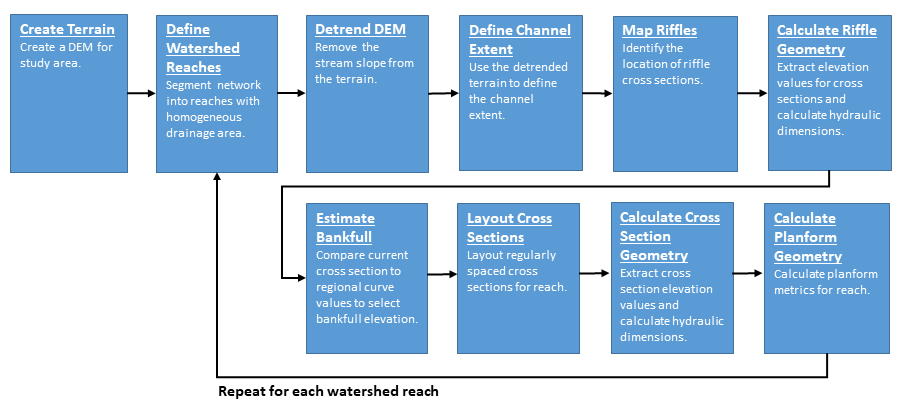
\includegraphics[width=1\linewidth]{images/Workflow_watershed} \caption{Workflow Diagram}\label{fig:unnamed-chunk-3}
\end{figure}

\section{Workflow Stages}\label{workflow-stages}

\begin{itemize}
\item
  Describe how the workflow is divided into stages and each stage
  contains steps.
\item
\end{itemize}

\subsection{Create Terrain}\label{create-terrain}

\begin{itemize}
\tightlist
\item
  What will be accomplished for each stage?
\item
  Describe how previous stage (outputs) flows into the current stage
  (inputs).
\end{itemize}

\subsection{Define Watershed Reaches}\label{define-watershed-reaches}

\subsection{Detrend DEM}\label{detrend-dem}

\subsection{Define Channel Extent}\label{define-channel-extent}

\subsection{Map Riffles}\label{map-riffles}

\subsection{Calculate Riffle Geometry}\label{calculate-riffle-geometry}

\subsection{Estimate Bankfull}\label{estimate-bankfull}

\subsection{Layout Cross Sections}\label{layout-cross-sections}

\subsection{Calculate Cross Section
Geometry}\label{calculate-cross-section-geometry}

\subsection{Calculate Planform
Geometry}\label{calculate-planform-geometry}

\chapter{Geoprocessing}\label{geoprocessing}

This section describes the geoprocessing steps required to extract
channel geomtery dimensions from a LiDAR derived digital elevation model
(DEM).

\section{Create Terrain}\label{create-terrain-1}

\subsection{Develop Elevation Model}\label{develop-elevation-model}

The purpose of this step is to develop a DEM for the study area.

\begin{itemize}
\tightlist
\item
  Obtain an off-the-shelf DEM for the study area.
\item
  Determine if sufficient resolution exists in the channel.
\item
  If not, assemble LAS data for the channel.
\item
  Create LAS dataset of study area.
\item
  Set the LAS Dataset projection to the coordinate system UTM (select
  appropriate Zone based on location of the study area), Datum: NAD83.
\item
  Select LAS classes that contain non-vegetation points within the
  channel.
\item
  Use the \texttt{LAS\ Dataset\ to\ Raster} tool to export to raster.

  \begin{itemize}
  \tightlist
  \item
    Z-Factor: 3.28084
  \item
    Cell assignment Type: IDW
  \item
    Void Fill Method: Natural Neighbor
  \item
    Cell size: 1 foot (0.3048 meters)
  \end{itemize}
\item
  Create a \texttt{study\_area} polygon feature class that delineates
  the extent of the study area. Use this feature class to clip the DEM
  to the desired study area. Edit this polygon to remove any elevation
  anomolies around the edges of the DEM. These anomolies are sometimes
  created by the \texttt{LAS\ Dataset\ to\ Raster} tool.
\end{itemize}

\subsection{Elevation Model Hydro
Modification}\label{elevation-model-hydro-modification}

The purpose of this step is to create a hydro-modified DEM to ensure
proper water flow across the study area.

\begin{itemize}
\tightlist
\item
  Examine the stream channel through the study area and determine if
  there are any blockages to flow in the DEM. These blockages are
  typically built infrastructure such as road embankments where streams
  are conveyed through culverts or underground stormwater structures.
\item
  If there are flow blockages in the study area, create a new line
  feature class named \texttt{cutlines} to store terrain modifications
  that remove flow blockages. This feature class must be in the same
  coordinate system as the DEM being modified.
\item
  In an edit session, identify human structures that block flow along
  the stream reach being studied. Draw a line beginning at the upstream
  side of the blockage to a point just downstream of the blockage.
\item
  Use the \texttt{02\ -\ Burn\ Cutlines} tool to ``burn'' the
  \texttt{cutlines} features into the DEM. This tool creates the
  \texttt{dem\_hydro} raster.
\end{itemize}

\section{Define Watershed Reaches}\label{define-watershed-reaches-1}

\subsection{Define Stream Reaches}\label{define-stream-reaches}

The purpose of this step is to create a synthetic flow network of
streams for the study area.

\begin{itemize}
\tightlist
\item
  Use the \texttt{03\ -\ Contributing\ Area} tool to calculate the
  contributing area for the study area. If created, use the
  \texttt{dem\_hydro} raster as input, otherwise use the original study
  area DEM. The \texttt{processes} parameter can be safely set to
  approximately 2 less than the number of cores on the computer running
  the tool.
\item
  Use the \texttt{04\ -\ Stream\ Network} tool to create a synthetic
  stream network from the hydro-modified DEM. The \texttt{processes}
  parameter can be safely set to approximately 2 less than the number of
  cores on the computer running the tool. The \texttt{threshold}
  parameter should be set to a value of 200,000 to 500,000 depending on
  the study area. If the resulting \texttt{stream\_network} is too dense
  (requiring a large amount of editing to remove extraneous
  tributaries), try rerunning the tool and increasing the
  \texttt{threshold} value. Conversely, if the resulting
  \texttt{stream\_network} is too sparse (not enough of the stream
  network was delineated), try rerunning the tool and decreasing the
  \texttt{threshold} value.
\item
  Edit the resulting \texttt{stream\_network} feature class to remove
  all tributary streams that do not constitute the network that will be
  analyzed in this study.
\item
  Edit the \texttt{stream\_network} feature class to ensure that stream
  segments are represented by a single line and that there are no gaps
  in the steam network.
\item
  Use the \texttt{Field\ Calculator} tool to set the \texttt{Name} field
  to the name of the site being analyzed. Failure to complete this step
  will cause the next tool run to fail.
\item
  Use the \texttt{05\ -\ Create\ Flowline} tool to process the
  \texttt{stream\_network} feature class that was just edited to produce
  a new \texttt{flowline} feature class. Use a smoothing tolerance from
  5-20. The goal is produce a smooth flowline, but not remove too much
  resolution from the line (ensure the line remains in the channel and
  not cut into the floodplain).
\item
  Edit the \texttt{flowline} feature class to ensure that the flowline
  is digitized beginning with the downstream end and digitized upstream.
  In an edit session, select the flowline, choose to edit vertices, and
  ensure that the red endpoint is at the upstream end of the flowline.
  Use the flip command to ensure flowline is digitized in the correct
  direction.
\end{itemize}

\subsection{Extract Stream Reach Profile
Points}\label{extract-stream-reach-profile-points}

The purpose of this step is convert the flowline into a series of points
along the stream. This tool takes the flowline feature class, converts
it to a route, calculates the distance to the mouth of the river for all
vertices, and creates a stream profile points feature class. The
flowline feature class was created during the hydro modification
process.

\begin{itemize}
\tightlist
\item
  Use the \texttt{06\ Stream\ Profile\ Points} tool to convert the
  \texttt{flowline} feature class into stream profile points. For this
  study, set the \texttt{km\_to\_mouth} parameter to 0 and the
  \texttt{station\_distance} field to 1 meter.
\end{itemize}

\section{Detrend DEM}\label{detrend-dem-1}

\subsection{Detrend Elevation Model}\label{detrend-elevation-model}

The purpose of this step is to produce a detrended DEM. A detrended DEM
normalizes stream bank elevations for a given reach.

\begin{itemize}
\tightlist
\item
  Use the \texttt{07\ -\ Detrend} tool to create a detrended DEM for the
  study reach. For this study, set the \texttt{buffer\_distance} field
  to 100 meters.
\end{itemize}

\section{Define Channel Extent}\label{define-channel-extent-1}

\subsection{Delineate the Initial Channel
Extent}\label{delineate-the-initial-channel-extent}

The purpose of this step is to use the detrended DEM to extract an
initial channel extent polygon.

\begin{itemize}
\tightlist
\item
  The \texttt{detrend} DEM created in the last step can be used to
  explore innundation extents at various water surface elevations. Add
  the \texttt{detrend} feature class to ArcMap. On the Symbology tab,
  use the Classified renderer to classify the raster into 2 classes. Set
  the first class boundary to the detrended elevation that you would
  like to explore. Set the color of the first class (min value -
  detrended elevation) to blue and the color of the second class
  (detrended elevation - max value) to No Color.
\item
  To delineate the channel extent, select a detrended elevation that
  innundates the channel up to at least the first terrace. The goal at
  this stage is to select a detrended elevation that captures the
  channel without going too far into the floodplain. Try several
  detrended elevation values to help make the decision.
\item
  When you have chosen a detrended elevation, use the
  \texttt{08\ -\ Bankfull\ Polygon} tool to extract a channel area
  polygon. This tool creas a new polygon feature class named
  \texttt{banks\_raw\_xxx}, where xxx is the detrended elevation
  selected.
\item
  This feature class must be edited to select the channel area
  polygon(s). Open the attribute table for the \texttt{banks\_raw\_xxx}
  feature class and use advanced sorting to sort first by
  \texttt{gridcode} and then by \texttt{Shape\_Area}. Polygons with
  \texttt{gridcode} = 1 are polygons innundated at the detrended
  elevation. Typically, the polygons with the largest area represent the
  channel. Begin selecting \texttt{gridcode} = 1 polygons with the
  largest area until the entire channel area is selected.
\item
  Export these selected features to a new feature class named
  \texttt{banks\_xxx}, where xxx is the detrended elevation selected.
\end{itemize}

\subsection{Create Channel Slope
Raster}\label{create-channel-slope-raster}

The purpose of this step is to create a channel slope raster that can be
used in the visual identification of riffe locations in following step.

\begin{itemize}
\tightlist
\item
  Use the \texttt{09\ -\ Channel\ Slope} tool to calculate a raster of
  the channel slope. This tool creates a new feature class named
  \texttt{channel\_slope}.
\end{itemize}

\section{Define Meander Loops}\label{define-meander-loops}

The purpose of this step is to delineate the meander loops and bends for
the stream reach.

\subsection{\texorpdfstring{Create the \texttt{banklines} feature
class}{Create the banklines feature class}}\label{create-the-banklines-feature-class}

The purpose of this step is to convert the \texttt{banks\_xxx} polygon
created in one of the previous steps into a feature class that has two
records, one representing the left descending bankline and another the
right descending bankline for the stream reach.

\begin{itemize}
\tightlist
\item
  Use the \texttt{Polygon\ To\ Line} tool to convert the
  \texttt{banks\_xxx} polygon feature class created in one of the
  previous steps into a line feature class named \texttt{banklines}.
\item
  Add a new string field to the \texttt{banklines} feature class named
  \texttt{ReachName}.\\
\item
  Add a new long integer field to the \texttt{banklines} feature class
  named \texttt{bank\_id}.
\item
  Add a new text field to the \texttt{banklines} feature class named
  \texttt{bank}. The purpose of this field is to designate which bank is
  the right descending bank and which is the left descending bank.
\item
  Start a new edit session on the \texttt{banklines} feature class.
\item
  Use the \texttt{Explode\ Multipart\ Feature} on the advanced editing
  toolbar to explode the multipart line feature.
\item
  Add the \texttt{flowline} feature class to the map document.
\item
  Use the \texttt{Split\ Tool} to split the line features at the end of
  the flowline. The banklines should not extend past the end of the
  flowline.
\item
  Use the `Split Tool' to trim any tributaries from the `banklines'
  feature class.
\item
  The goal of this step is to have only two features, one representing
  the left descending bankline and another the right descending
  bankline. Delete all other line features.
\item
  Ensure that the banklines are digitized in the upstream direction.
  Edit the \texttt{banklines} feature class to ensure that each bankline
  is digitized beginning with the downstream end and digitized upstream.
  In an edit session, select the flowline, choose to edit vertices, and
  ensure that the red endpoint is at the upstream end of each bankline.
  Use the flip command to ensure each bankline is digitized in the
  correct direction.
\item
  In the \texttt{ReachName} field enter the reach name.
\item
  In the \texttt{bank} field, enter the string
  \texttt{right\ descending} or \texttt{left\ descending} to designate
  which bank each line represents.
\item
  In the \texttt{bank\_id} field enter a \texttt{1} for the
  \texttt{right\ descending} bank and \texttt{2} for the
  \texttt{left\ descending} bank.
\end{itemize}

\subsection{\texorpdfstring{Create the \texttt{loop\_points} feature
class}{Create the loop\_points feature class}}\label{create-the-loop_points-feature-class}

The purpose of this step is to create a point feature class to delineate
the start, end, and apex of each meander loop and bend.

\begin{itemize}
\tightlist
\item
  Create a new point feature class named \texttt{loop\_points}. Enable z
  and m values. The feature class should contain the following fields:

  \begin{itemize}
  \tightlist
  \item
    \texttt{loop} - long integer
  \item
    \texttt{bend} - long integer
  \item
    \texttt{position} - text (10)
  \item
    \texttt{ReachName} - text (50)
  \end{itemize}
\item
  Begin numbering loops and bends starting at the downstream end of the
  reach and increase numbering upstream.
\item
  Instructions for placing points goes here.
\end{itemize}

\section{Define Valley Line}\label{define-valley-line}

The purpose of this step is to define a line that represents the trend
of the valley for the stream reach.

\begin{itemize}
\tightlist
\item
  The \texttt{flowline} feature class will be generalized to create the
  \texttt{valleyline} feature class. This will be an iterative process
  of generating a new smoothed line and comparing it with the
  \texttt{loop\_points} feature class. The goal is to find the smooth
  line that passses through the defined meander loops.
\item
  Use the \texttt{Smooth\ Line} tool to smooth the \texttt{flowline}
  feature class. Use the \texttt{PAEK} smoothing algorithm. Start with a
  smoothing tolarance value of 100 meters. Name the output feature class
  \texttt{valleyline\_100}
\item
  Check how well the new smoothed \texttt{valleyline\_100} feature class
  passes through the meander loops defined in \texttt{loop\_points}. If
  the fit is unacceptable, try increasing the smoothing tolerance value.
\item
  Try a range of smoothing tolerances to generate a set of valleylines.
\item
  The ideal smoothed valleyline should:

  \begin{itemize}
  \tightlist
  \item
    Divide loop apex values in an alternating pattern (required)
  \item
    Cross the flowline at the inflection points between meander loops
    (ideal)
  \end{itemize}
\item
  Select the smoothed line with the best fit. Delete the unselected
  smoothed lines. Rename the selected smoothed line \texttt{valleyline}.
\end{itemize}

\section{Map Riffles}\label{map-riffles-1}

The purpose of this step is to identify and map riffe locations. Riffles
will be used in later steps to determine the bankfull elevation from
gage stage discharge relationships.

\subsection{Map Riffle Cross Sections}\label{map-riffle-cross-sections}

Riffle locations are identified using the \texttt{channel\_slope} raster
calculated in the last step (and confirmed with high resolution aerial
imagery). In the \texttt{channel\_slope} raster, pools appear as
relatively smooth areas of low slope due to the absence of LiDAR points
(deep water absorbs laser pulses). Shallow water riffles appear as
highly textured areas of relatively higher slope between pools due to
the higher number of LiDAR points from the exposed bed material.

\begin{itemize}
\item
  Create a new line feature class named \texttt{riffle} to store riffle
  cross sections. This feature class must be in the same coordinate
  system as the DEM.
\item
  Riffle locations should have the following characteristics:

  \begin{itemize}
  \tightlist
  \item
    A straight reach between two meander bends, areas in the cross-overs
    between river bends
  \item
    Clear indicators of of the active floodplain or bankfull discharge
  \item
    Presence of one or more terraces
  \item
    Channel section and form typical of the stream
  \item
    A reasonably clear view of of geomorphic features
  \item
    Areas of high water surface slope
  \item
    Areas of minimum depth and width
  \item
    Channel width parallel and consistent
  \item
    Avoid tributary influences
  \end{itemize}
\item
  Digitize cross sections beginning with the left descending bank. In an
  edit session, use the flip command to ensure cross sections are
  digitized in the correct direction. A red vertex denotes the end of a
  line segment.
\item
  Ensure that cross sections are digitized to a detrended elevation of
  at least 108 to 112 feet. Use the raster classification technique
  described above (Bankfull Polygon section) to explore innundation
  extents to identify this maximum detrended elevation that riffle cross
  sections should delineated to.
\item
  Since riffle cross sections should be delineated in locations where
  there are clear indicators of of the active floodplain or bankfull
  discharge, ensure that riffle cross sections include at least a
  portion of the adjacent floodplain. Including at least a portion of
  the adjacent floodplain allows a fluvial geomorphologist the ability
  to examine the elevation of the floodplain. Including a 20- to 50-feet
  section should be sufficient.
\end{itemize}

\section{Calculate Riffle Geometry}\label{calculate-riffle-geometry-1}

\subsection{Assign Cross Section IDs}\label{assign-cross-section-ids}

The purpose of this step is to ensure that cross section identifiers are
properly assigned to allow later tools to run correctly.

\begin{itemize}
\tightlist
\item
  Add a long integer field named \texttt{Seq} to the \texttt{riffle}
  feature class to hold the unique number of the cross section. This
  will be used to iterate through cross sections.
\item
  Assign integer values to the \texttt{Seq} field starting with one.
  Begin numbering at the downstream extent of the study area and moving
  upstream.
\end{itemize}

\subsection{Calculate Cross Section Watershed
Area}\label{calculate-cross-section-watershed-area}

The purpose of this step is calculate the watershed area of each cross
section. The watershed area draining to each cross section will be used
in later steps to define several hydraulic geometry relationships.

\begin{itemize}
\tightlist
\item
  Add the NHDPlus flow accumulation \texttt{NHDPlus\_FAC} that has been
  clipped to the study region to an ArcMap document. Measure the
  distance from the flowline to each cross section to determine the snap
  distance required.
\item
  Use the \texttt{12\ -\ XS\ Watershed\ Area} tool to calculate the
  watershed area for each cross section.
\end{itemize}

\subsection{Assign Cross Section River
Position}\label{assign-cross-section-river-position}

The purpose of this step is to assign a river position to each cross
section. The river position of each cross section will be used in later
steps to calculate several channel parameters (i.e., gradient,
sinuosity).

\begin{itemize}
\tightlist
\item
  Use the \texttt{13\ -\ XS\ Assign\ River\ Position} tool to calculate
  the distance to the mouth of the river for each cross section.
\end{itemize}

\subsection{Calculate Cross Section Station
Points}\label{calculate-cross-section-station-points}

The purpose of this step is convert the cross section line feature class
into a point feature class representing cross section station points.
This feature class will be used in later steps to calculate hydraulic
geometry dimensions.

\begin{itemize}
\tightlist
\item
  Use the \texttt{14\ -\ XS\ Create\ Station\ Points} tool to calculate
  cross section station points for each cross section. For this study,
  set the \texttt{station\_distance} parameter to 0.3048 meter (1 foot).
  This tool creates a new feature class named
  \texttt{cross\_section\_points}.
\item
  Export the \texttt{cross\_section\_points} feature class attribute
  table to a text file named
  \texttt{\textless{}study\_area\textgreater{}\_cross\_section\_points.csv},
  where \texttt{\textless{}study\_area\textgreater{}} is the name of the
  study area.
\end{itemize}

\subsection{Check Cross Sections}\label{check-cross-sections}

The purpose of this step is to plot each cross section to ensure it was
digitized correctly.

\begin{itemize}
\tightlist
\item
  Use the \texttt{15\ -\ XS\ Plot} tool to plot each riffle cross
  section. Make an educated guess at the value of
  \texttt{bankfull\_elevation} for the purpose of this QA check.
\item
  After creating a plot of the first cross section, in the
  \texttt{R\ Graphics} window, turn on recording
  (\texttt{History\textbar{}Recording}) to keep a record of the
  subsequent cross section plots created during this session. Use the
  keyboard's \texttt{Page\ Up} and \texttt{Page\ Down} keys to scroll
  through the plots. If you make a mistake, use the
  \texttt{History\textbar{}Clear\ History} menu item to clear the
  previously recorded graphs.
\item
  Use the plots to check that the digitized cross sections have the
  following characteristics:

  \begin{itemize}
  \tightlist
  \item
    Banks should be digitized to a high enough elevation sufficient to
    contain the anticipated bankfull elevation. This is typically
    between a detrended elevation of 108 to 112 feet. However, do not
    exceed this elevation as it will reduce the resolution of the
    geomorphic features within the the channel displayed on the graph.
  \item
    Left and right banks are digitized to a similar elevation. One bank
    should not be extremely higher that the other.
  \item
    A geomorphologist will provide you with feedback on the bankfull
    elevation and maximum elevation to use for each stream reach. As a
    result, the cross section digitizing process will necessarily be
    iterative based on feedback from a fluvial geomorphologist.
  \item
    Ensure that cross sections are digitized into a portion of the
    adjacent floodplain. Cross sections should extend 20 to 50 feet into
    the floodplain.
  \end{itemize}
\end{itemize}

\section{Estimate Bankfull}\label{estimate-bankfull-1}

\section{Layout Cross Sections}\label{layout-cross-sections-1}

\section{Calculate Cross Section
Geometry}\label{calculate-cross-section-geometry-1}

\section{Calculate Planform
Geometry}\label{calculate-planform-geometry-1}

\chapter{Examples}\label{examples}

Worked examples are demonstrated in this chapter using tutorial data.

\section{Select Region}\label{select-region}

\section{Process Gage One}\label{process-gage-one}

\section{Calculate Regional Curve}\label{calculate-regional-curve}

\chapter{Summary}\label{summary}

The concluding chapter is the last chapter in the main body of the
report before the reference list. The title and content may vary
depending on the project type and audience. The chapter is usually
called ``Summary,'' ``Conclusions,'' or ``Conclusions and
Recommendations.''

A technical report may conclude with a summary chapter if its purpose is
to document empirical observations or straightforward research findings
such as the results of a field demonstration or a laboratory test
series. A summary typically reviews the research results in more detail
than the abstract.

A chapter of conclusions differs from a summary chapter in that it
presents or reviews the author's technical interpretation of the
research results. Conclusions concisely help the reader to understand
how the research objective was met and what the results mean in terms of
the Army problem described in the background section. Conclusions should
be included for every secondary objective stated in the introductory
chapter.

Most reports will include recommendations for the project sponsor.
Recommendations generally will pertain to (1) how the research product
or results should be used to address the problem defined in the first
chapter or (2) what the sponsor may do to transition a technology
product into advanced development, field demonstration, or
commercialization.

A reference list is presented immediately after the final numbered
chapter of the report, but before any appendixes. Formats and styles
prescribed in the Chicago Manual of Style should be used. Most ERDC
reports will use the author-date system and corresponding reference list
form described in the Chicago Manual. An alternative style prescribed in
the Chicago Manual, the note-bibliography system, may be used by authors
working in disciplines in which that style is customary.

The reference list should include every information source cited in text
plus any uncited sources that were drawn upon. The reference list for
this Guide, presented on page 28, may be used as a model for common
types of source documentation including books, serial publications,
government documents, and unpublished material.

\chapter*{Mapping Riffles}\label{mapping-riffles}
\addcontentsline{toc}{chapter}{Mapping Riffles}

\bibliography{book.bib,packages.bib}


\end{document}
